\documentclass[tikz]{standalone}% 'crop' is the default for v1.0, before it was 'preview'
\usetikzlibrary{positioning,matrix,shapes,arrows,calc}

\pgfdeclareimage[height=1cm]{ngreen}{img/ngreen.pdf}
\pgfdeclareimage[height=1cm]{nblue}{img/nblue.pdf}
\pgfdeclareimage[height=1cm]{nred}{img/nred.pdf}
\pgfdeclareimage[height=1cm]{nblack}{img/nblack.pdf}

%\usetikzlibrary{...}% tikz package already loaded by 'tikz' option
\begin{document}
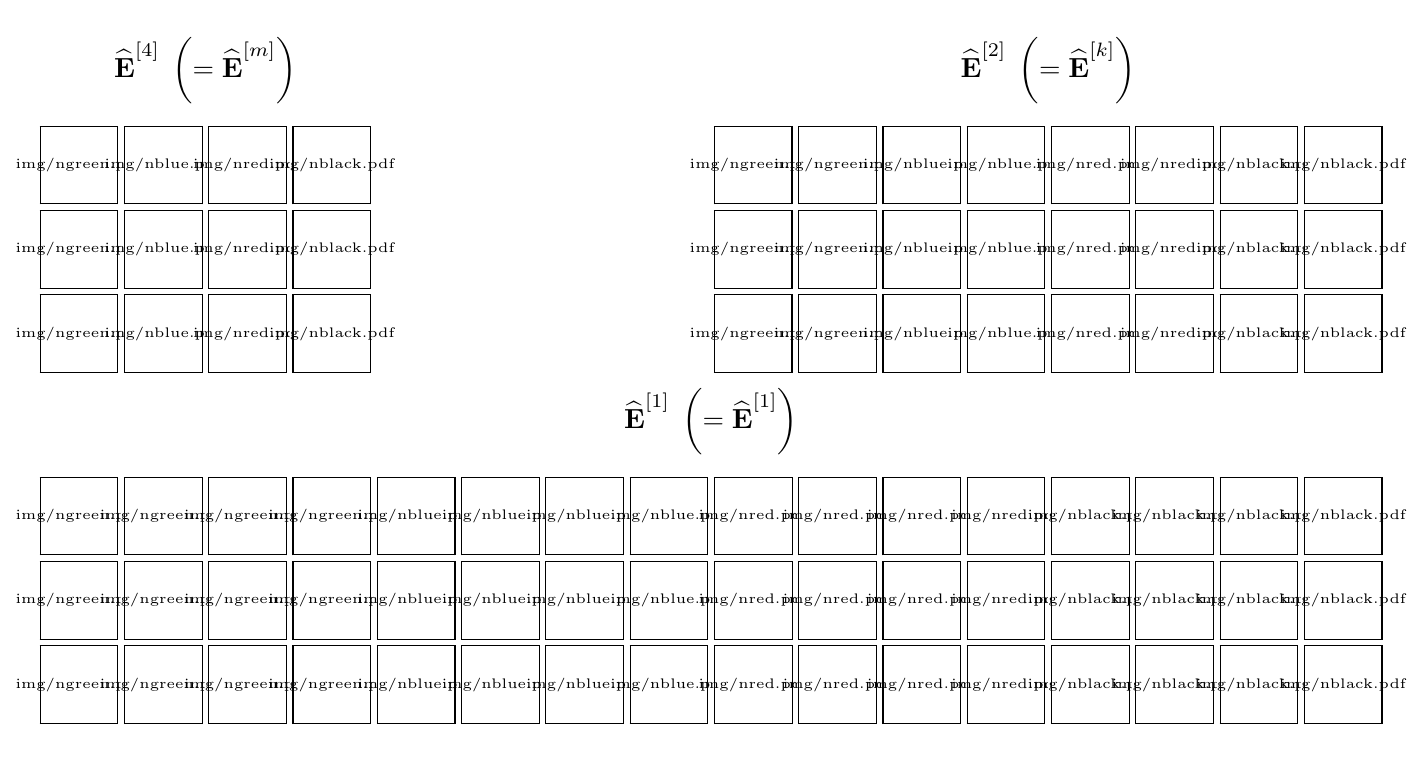
\begin{tikzpicture}
\matrix (e1) [matrix of nodes,row sep=0cm,column sep=0cm, nodes= {rectangle, fill=white, inner sep = 1pt}, label=above:{$\widehat{\textbf{E}}^{[1]}\;\left(=\widehat{\textbf{E}}^{[1]}\right)$}]
{
\pgfuseimage{ngreen} & \pgfuseimage{ngreen} & \pgfuseimage{ngreen} & \pgfuseimage{ngreen} & \pgfuseimage{nblue} & \pgfuseimage{nblue}  & \pgfuseimage{nblue} & \pgfuseimage{nblue} & \pgfuseimage{nred} & \pgfuseimage{nred} & \pgfuseimage{nred} & \pgfuseimage{nred} & \pgfuseimage{nblack} & \pgfuseimage{nblack} & \pgfuseimage{nblack} & \pgfuseimage{nblack}\\
\pgfuseimage{ngreen} & \pgfuseimage{ngreen} & \pgfuseimage{ngreen} & \pgfuseimage{ngreen} & \pgfuseimage{nblue} & \pgfuseimage{nblue}  & \pgfuseimage{nblue} & \pgfuseimage{nblue} & \pgfuseimage{nred} & \pgfuseimage{nred} & \pgfuseimage{nred} & \pgfuseimage{nred} & \pgfuseimage{nblack} & \pgfuseimage{nblack} & \pgfuseimage{nblack} & \pgfuseimage{nblack}\\
\pgfuseimage{ngreen} & \pgfuseimage{ngreen} & \pgfuseimage{ngreen} & \pgfuseimage{ngreen} & \pgfuseimage{nblue} & \pgfuseimage{nblue}  & \pgfuseimage{nblue} & \pgfuseimage{nblue} & \pgfuseimage{nred} & \pgfuseimage{nred} & \pgfuseimage{nred} & \pgfuseimage{nred} & \pgfuseimage{nblack} & \pgfuseimage{nblack} & \pgfuseimage{nblack} & \pgfuseimage{nblack}\\
};

\matrix (ek) [above= 10mm of e1.north east,
       anchor=south east, matrix of nodes,row sep=0cm,column sep=0cm, nodes= {rectangle, fill=white, inner sep = 1pt}, label=above:{$\widehat{\textbf{E}}^{[2]}\;\left(=\widehat{\textbf{E}}^{[k]}\right)$}]
{
\pgfuseimage{ngreen} & \pgfuseimage{ngreen} & \pgfuseimage{nblue} & \pgfuseimage{nblue} & \pgfuseimage{nred} & \pgfuseimage{nred} & \pgfuseimage{nblack} & \pgfuseimage{nblack}\\
\pgfuseimage{ngreen} & \pgfuseimage{ngreen} & \pgfuseimage{nblue} & \pgfuseimage{nblue} & \pgfuseimage{nred} & \pgfuseimage{nred} & \pgfuseimage{nblack} & \pgfuseimage{nblack}\\
\pgfuseimage{ngreen} & \pgfuseimage{ngreen} & \pgfuseimage{nblue} & \pgfuseimage{nblue} & \pgfuseimage{nred} & \pgfuseimage{nred} & \pgfuseimage{nblack} & \pgfuseimage{nblack}\\
};

\matrix (em) [above= 10mm of e1.north west,
       anchor=south west, matrix of nodes,row sep=0cm,column sep=0cm, nodes= {rectangle, fill=white, inner sep = 1pt}, label=above:{$\widehat{\textbf{E}}^{[4]}\;\left(=\widehat{\textbf{E}}^{[m]}\right)$}]
{
\pgfuseimage{ngreen} & \pgfuseimage{nblue} & \pgfuseimage{nred} & \pgfuseimage{nblack}\\
\pgfuseimage{ngreen} & \pgfuseimage{nblue} & \pgfuseimage{nred} & \pgfuseimage{nblack}\\
\pgfuseimage{ngreen} & \pgfuseimage{nblue} & \pgfuseimage{nred} & \pgfuseimage{nblack}\\
};
\end{tikzpicture}
\end{document}
